
\chapter{Motion along a Straight Line}

\section{Discussion Questions}

% 2.1
\discussion{Speed.  Velocity has a direction as well as a magnitude.}

% 2.2
\discussion{Since the dots appear to be increasing by what appears a multiple of the previous distance I would say it is graph (d).}

% 2.3
\discussion{Yes, if the velocity and acceleration have ``different signs''.  This is because the velocity is ``slowing down'' and will eventually reach zero, then start ``increasing again''.  You can also look at the formula for velocity with constant acceleration to see why.  It cannot reverse twice though as a straight line cannot pass through the x-axis twice.}

% 2.4
\discussion{Either when the velocity is constant or special cases when the acceleration changes direction and after a period of time the average velocity will match the instantaneous velocity.}

% 2.5
\discussion{ (b) Yes.  When the velocity and acceleration are in ``opposite directions''.  Yes, if they both point in the ``same direction''.}

% 2.6
\discussion{Constant acceleration.  Anytime you start from 0 speed and accelerate then end up at 0 speed will the speed equal the magnitude of the velocity at some point.}

% 2.7
\discussion{Average velocities are the same but in opposite directions.}

% 2.8
\discussion{You could argue that you would be able to ticket all parked cars that people who speed pass by.}

% 2.9
% This question is no very clear.  I assume they mean instantaneous velocity when they say velocity.
\discussion{No, because displacement is 0, $\Delta{x}$ = zero, then by definition the average velocity is 0.  For the second yes;  $x =sin(t)$, then $y=cos(t)$.  When t = 0 displacement is 0 but velocity is 1.}

% 2.10
\discussion{Yes. If you assume the object is already moving and there is no acceleration then the object will keep moving.}

% 2.11
\discussion{180km/hr * 1h/60m * 1m = 3km. 6.0 seconds is 1/10th of a minute, so 1/10th of 3km, 0.3km}

% 2.12
\discussion{360km/hr, since this is linear half the time means twice the speed.}

% 2.13
\discussion{(a) one being a straight line and the other being a parabola going throught the two points.  (b) Average V is $\delta{x}/\delta{t}$ so same for both.}

% 2.14
\discussion{No.  Imagine the top half of a circle starting a 0~\si{\meter/\second} and ending with 0~\si{\meter/\second}, the average would be 0, which it obviously isn't.}

% 2.15
\discussion{Thrown.  The distance travelled to go from 0 to the starting speed is more than the distance from your hand to the top.  If you calculate the acceleration you can see that in your hand is higher.}

% 2.16
\discussion{Your friend will beat you, it takes you $\frac{21}{20}~\si{\hour}$ and your friend $\frac{3}{5}~\si{\hour}$.}

% 2.17
\discussion{-9.8\si{\meter/\second^2}, it starts at that value but decreases over time.}

% 2.18
\discussion{The elevator.}

% 2.19
\discussion{(a) Same speed (b) Ball thrown down (c) Same (d) Ball thrown up }

% 2.20
\discussion{Less than 4~\si{\meter/\second}}

% 2.21
\discussion{Velocity is 0, and it is changing.  This change is the acceleration.}

% 2.22
\discussion{$\sqrt(3)T$}

\section{Exercises}

\subsection*{Displacement, Time, and Average Velocities}

% 2.1
\exercise{32.9~\distance}

% 2.2
\exercise{(a) -0.00476~\si{\meter/\second} (b) 0~\si{\meter/\second}}

% 2.3
\exercise{1.38 hours longer}

% 2.4
\exercise{(a) 4.4~\si{\meter/\second} (b) -7.3~\si{\meter/\second}}

% 2.5
\exercise{(a) 0.28~\si{\meter/\second} (b) 1.25~\si{\meter/\second}}

% 2.6
\exercise{(a) 2.74~\si{\meter/\second} (b) 4.94~\si{\meter/\second} (c) 7.40~\si{\meter/\second}}

\subsection*{Instantaneous Velocity}

% 2.7
\exercise{(a) 41~\si{\meter/\second} (b) v(0) = 21.8~\si{\meter/\second} v(10) = 27~\si{\meter/\second}}

% 2.8
\exercise{3.62~\si{\meter/\second}}

% 2.9
\exercise{(a) $\frac{7}{3}$~\si{\meter/\second}, same for both (b) $V_{avg} = \frac{1}{3}$~\si{\meter/\second} $Speed_{avg} = \frac{7}{3}$~\si{\meter/\second} }

% 2.10
\exercise{(a) \rom{4} (b) \rom{1} (c) \rom{5} (d) \rom{2} (e) none }

% 2.11
\exercise{A: $\frac{20}{3}$~\velocity B: $\frac{20}{3}$~\velocity C: $0$~\velocity D: $-40$~\velocity}

\subsection*{Average and Instantaneous Acceleration}

% 2.12
\exercise{
(a) (i) 6~\acceleration (ii) -6~\acceleration (iii) 0~\acceleration (iv) 0~\acceleration \\
(b) 0~\acceleration and -6~\acceleration
}

\begin{figure}[!ht]
    \centering
    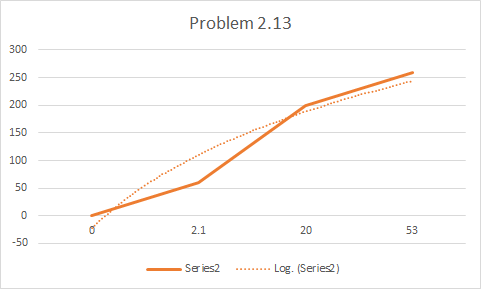
\includegraphics[scale=0.5]{mechanics/chapter2/problem2.13Speed.png}
    \caption{Problem 2.13}
    \label{fig:Problem2.13}
\end{figure}


% 2.13
\exercise{
(a) \Fig{fig:Problem2.13} \\
(b) (i) $28.6~\acceleration$ (ii) $7.82~\acceleration$ (iii) $1.82~\acceleration$
}

% 2.14
\exercise{6.93~\acceleration}

\begin{figure}[ht!]
    \begin{minipage}{.5\linewidth}
    \centering
    \subfloat[Position]{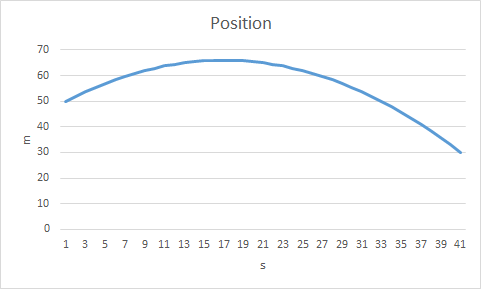
\includegraphics[scale=0.45]{mechanics/chapter2/problem2.15Position.png}\label{fig:Problem2.15Position}}
    \end{minipage}%
    \begin{minipage}{.5\linewidth}
    \centering
    \subfloat[Velocity]{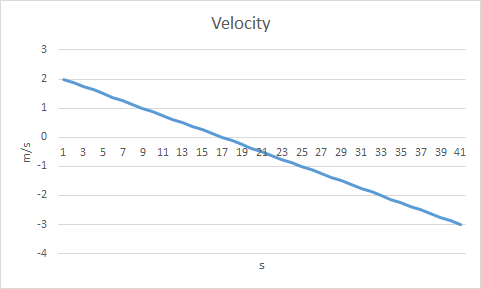
\includegraphics[scale=0.45]{mechanics/chapter2/problem2.15Velocity.png}\label{fig:Problem2.15Velocity}}
    \end{minipage}\par\medskip
    \centering
    \subfloat[Acceleration]{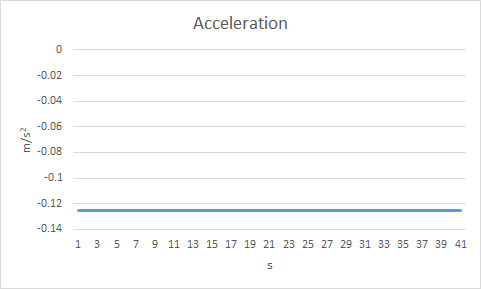
\includegraphics[scale=0.45]{mechanics/chapter2/problem2.15Acceleration.png}\label{fig:Problem2.15Acceleration}}

    \caption{Problem 2.15}
    \label{fig:Problem2.15}
\end{figure}

% 2.15
\exercise{(a) 2.00~\si{\centi\meter/\second} 50.0~\si{\centi\meter} 0.125~\si{\centi\meter/\second^2} \\
(b) 16~\si{\second} \\
(c) 32~\si{\second} \\
(d) -13.9~\si{\second} and 45.9~\si{\second} \\
(e) \Fig{fig:Problem2.15}
}

% 2.16
\exercise{
(a) mag: 0.963~\acceleration sign: positive dir: right \\
(b) mag: 0.963~\acceleration sign: negative dir: left  \\
(c) mag: 2.83~\acceleration  sign: negative dir: left
}

\begin{figure}[ht!]
    \begin{minipage}{.5\linewidth}
        \centering
        \subfloat[Position]{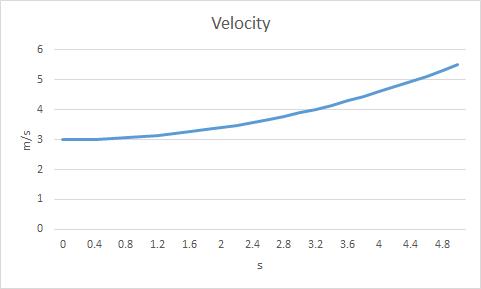
\includegraphics[scale=0.45]{mechanics/chapter2/problem2.17Velocity.png}\label{fig:Problem2.17Velocity}}
    \end{minipage}%
    \begin{minipage}{.5\linewidth}
        \centering
        \subfloat[Velocity]{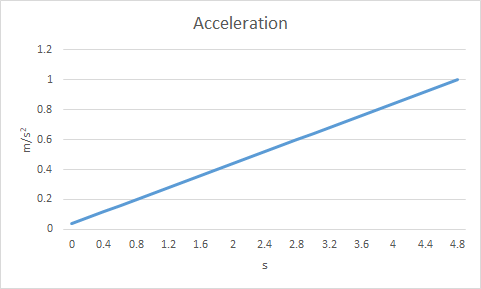
\includegraphics[scale=0.45]{mechanics/chapter2/problem2.17Acceleration.png}\label{fig:Problem2.17Acceleration}}
    \end{minipage}\par\medskip

    \caption{Problem 2.17}
    \label{fig:Problem2.17}
\end{figure}

% 2.17
\exercise{ 
(a) $0.5~\acceleration$ (b) \Fig{fig:Problem2.17}
}

\begin{figure}[ht!]
    \begin{minipage}{.5\linewidth}
    \centering
    \subfloat[Position]{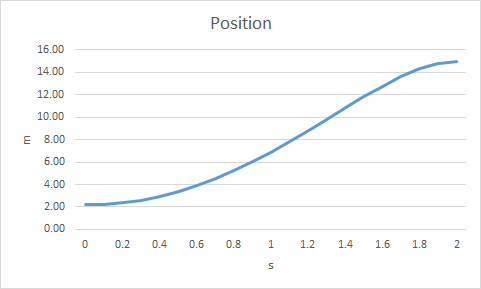
\includegraphics[scale=0.45]{mechanics/chapter2/problem2.18Position.png}\label{fig:Problem2.18Position}}
    \end{minipage}%
    \begin{minipage}{.5\linewidth}
    \centering
    \subfloat[Velocity]{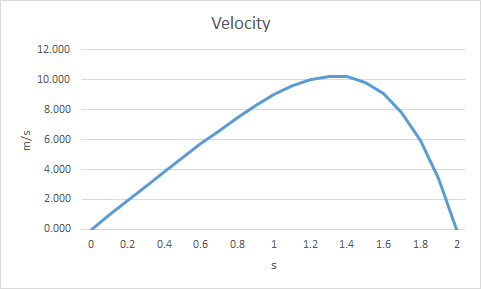
\includegraphics[scale=0.45]{mechanics/chapter2/problem2.18Velocity.png}\label{fig:Problem2.18Velocity}}
    \end{minipage}\par\medskip
    \centering
    \subfloat[Acceleration]{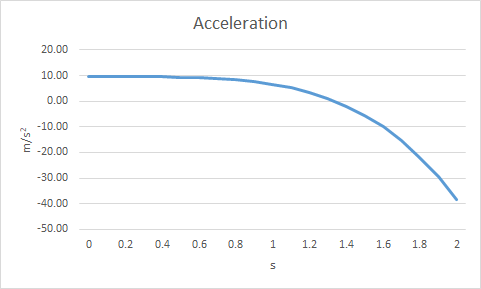
\includegraphics[scale=0.45]{mechanics/chapter2/problem2.18Acceleration.png}\label{fig:Problem2.18Acceleration}}

    \caption{Problem 2.18}
    \label{fig:Problem2.18}
\end{figure}

% 2.18
\exercise{
(a) t = 0 x = 2.17\distance, t=+2 x = 15\distance, t=-2 x = 15\distance \\
(b) \Fig{fig:Problem2.18}
}

\subsection*{Motion with constant Acceleration}

% 2.19
\exercise{(a) 5.40~\velocity (b) 1.36~\acceleration}

% 2.20
\exercise{ (a) Yes (b) 245~\velocity}

% 2.21
\exercise{736~\acceleration}

% 2.22
\exercise{(a) 2500~\acceleration (b) 1.06~\distance}

% 2.23
\exercise{1.55~\distance}

% 2.24
\exercise{(a) 33.8~\si{\second} (b) 662~\distance}

% 2.25
\exercise{0.38~\distance}

% 2.26
\exercise{(a) -39~\acceleration (b) 0.018~\si{\second}}

% 2.27
\exercise{(a) 3.13e6~\acceleration (b) 0.016~\si{\second} (c) No}

% 2.28
\exercise{ (a) 1.4~\velocity (b) 13~\si{\second} (c) 234~\distance}

% 2.29
\exercise{
(a) (i) 7.11e4\si{\kilo\meter/\hour^2} (ii) 9.84e4\si{\kilo\meter/\hour^2} \\
(b) (i) 0.18~\si{\kilo\meter} (ii) 13~\si{\kilo\meter}
}

\section{Problems}

\section{Challenge Problems}